\documentclass[11pt, fleqn]{article}
\usepackage[a4paper, hmargin={2.8cm, 2.8cm}, vmargin={2.5cm, 2.5cm}]{geometry}  % Geometri-pakke: Styrer bl.a. maginer    %
%%%%%%%%%%%%%%%%%%%%%%%%%%%%%%%%%%%%%%%%%%%%%%%%%%%%%%%%%%%%%%%%%%%%%%%%%
\usepackage[babel, stor, da]{ku-forside} % KU-forside
\usepackage[utf8]{inputenc}
\usepackage{listings}
\usepackage{amsmath}
\usepackage{amsfonts}
\usepackage{graphicx}
\usepackage[hidelinks]{hyperref}
\usepackage{pdfpages}
\usepackage{float}
\usepackage{maplestd2e}
\def\emptyline{\vspace{12pt}}
%
% Mini-manual til ku-forside pakken:
%
% Sprogmuligheder:     da, en
% babel loader babelpakken, med det valgte sprog
% Fakultetsmuligheder: farma, hum, jur, ku, life, nat, samf, sund, teo
% Farvemuligheder:     sh, farve
% Forsidemuligheder: lille, stor, titelside
%      titelside er identisk med designet på ku.dk/designmanual
%      lille er giver et lille logo sammen med titlen på den første side
%      stor er giver et stort logo sammen med titlen på den første side
%
% Default er [da,nat,farve,titelside]
%
% Ex. \usepackage[babel, lille, jur, sh, en]{ku-forside} giver et lille logo i sorthvid for juridisk fakultet og loader babelpakken med engelsk som sprog.

%%%%%%%%%%%%%%%%%%%%%%%%%%%%%%%%%%%%%%%%%%%%%%
%%%               Titel                    %%%
%%%%%%%%%%%%%%%%%%%%%%%%%%%%%%%%%%%%%%%%%%%%%%
\titel{MatIntro} %
\undertitel{Pointopgave 4} %
%\opgave{Overspringshandling} % Findes kun under 'titelside'
\forfatter{Jesper Henrichsen | tgw831}%
\dato{\today}%
%\vejleder{Doktoren} %  Findes kun under 'titelside'
%%%%%%%%%%%%%%%%%%%%%%%%%%%%%%%%%%%%%%%%%%%%%%%%%%%%%%%%%%%%%%%%%%
%%%                 Her begynder dokumentet                    %%%
%%%%%%%%%%%%%%%%%%%%%%%%%%%%%%%%%%%%%%%%%%%%%%%%%%%%%%%%%%%%%%%%%%
\begin{document}
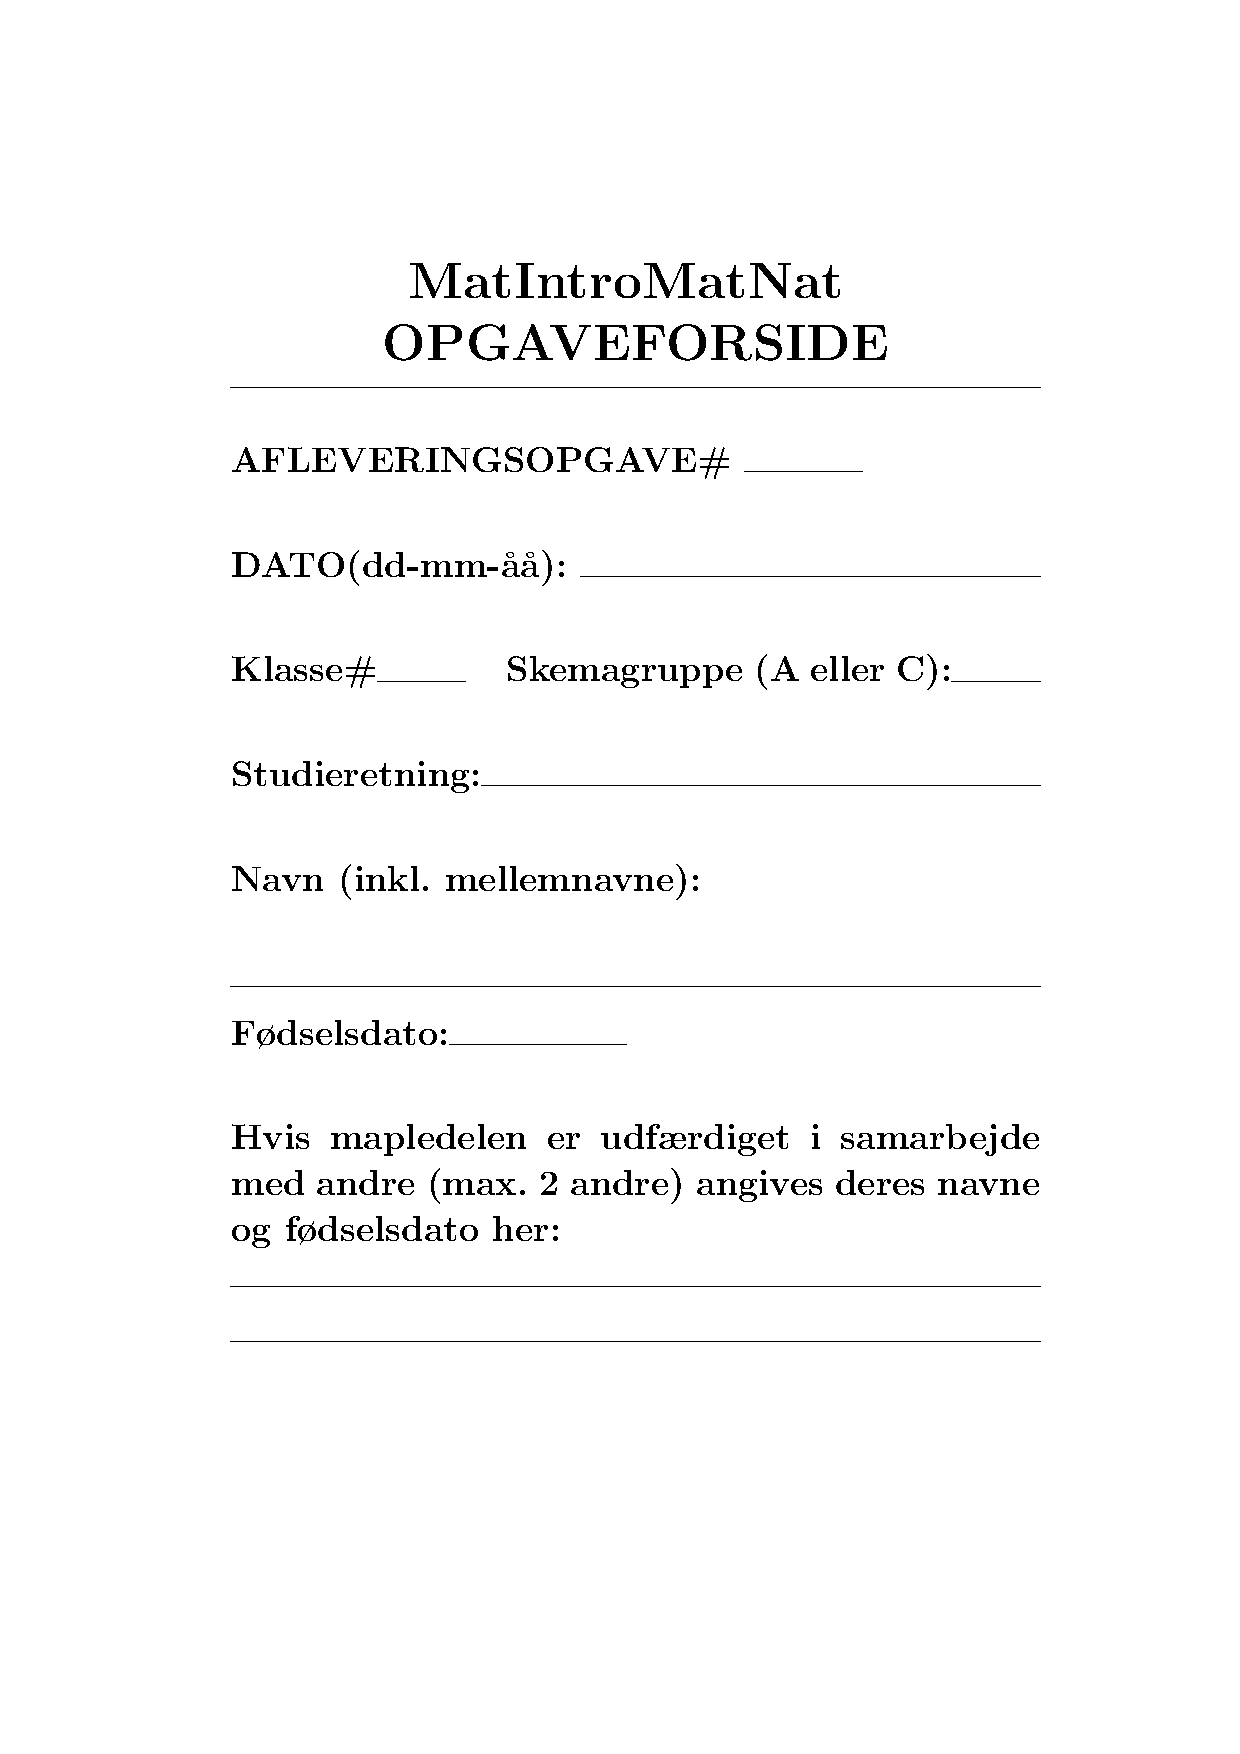
\includepdf[pages=-]{forside.pdf}
\maketitle % LAVER TITLEN
%\newpage
%%%%%%%%%%%%%%%%%%%%%%%%%%%%%%%%%%%%%%%%%%%%%%%%%%%%%%%%%%%%%%%%
%%%%%%%%%%%%%%%%%%%% TEKST BEGYNDER HER  %%%%%%%%%%%%%%%%%%%%%%%
%%%%%%%%%%%%%%%%%%%%%%%%%%%%%%%%%%%%%%%%%%%%%%%%%%%%%%%%%%%%%%%%
\section*{4.1}

\begin{equation}
\label{eq:4_1}
(1+x^2)yy'=x(1+y^2)
\end{equation}
Først ved løsning i Maple fås:
%\newpage
\begin{figure}[H]
\caption{Maple input og output}
\begin{center}
%% Created by Maple 2015.1, Linux
%% Source Worksheet: 4_1_maplesolve.mw
%% Generated: Tue Sep 22 23:08:01 CEST 2015

\pagestyle{empty}
\DefineParaStyle{Maple Heading 1}
\DefineParaStyle{Maple Text Output}
\DefineParaStyle{Maple Dash Item}
\DefineParaStyle{Maple Bullet Item}
\DefineParaStyle{Maple Normal}
\DefineParaStyle{Maple Heading 4}
\DefineParaStyle{Maple Heading 3}
\DefineParaStyle{Maple Heading 2}
\DefineParaStyle{Maple Warning}
\DefineParaStyle{Maple Title}
\DefineParaStyle{Maple Error}
\DefineCharStyle{Maple Hyperlink}
\DefineCharStyle{Maple 2D Math}
\DefineCharStyle{Maple Maple Input}
\DefineCharStyle{Maple 2D Output}
\DefineCharStyle{Maple 2D Input}
\mapleinline{inert}{2d}{DF := (x^2+1)*y(x)*(diff(y(x), x)) = x*(1+y(x)^2)}{\[\displaystyle {\it DF}\, := \, \left( {x}^{2}+1 \right) y \left( x \right) {\frac {\rm d}{{\rm d}x}}y \left( x \right) =x \left( 1+ \left( y \left( x \right)  \right) ^{2} \right) \]}
\begin{maplegroup}
\mapleresult
\begin{maplelatex}
\mapleinline{inert}{2d}{(x^2+1)*y(x)*(diff(y(x), x)) = x*(1+y(x)^2)}{\[\displaystyle  \left( {x}^{2}+1 \right) y \left( x \right) {\frac {\rm d}{{\rm d}x}}y \left( x \right) =x \left( 1+ \left( y \left( x \right)  \right) ^{2} \right) \]}
\end{maplelatex}
\end{maplegroup}
\mapleinline{inert}{2d}{dsolve(DF); 1}{\[\displaystyle {\it dsolve(DF);} \]}
\begin{maplegroup}
\mapleresult
\begin{maplelatex}
\mapleinline{inert}{2d}{y(x) = sqrt(_C1*x^2+_C1-1), y(x) = -sqrt(_C1*x^2+_C1-1)}{\[\displaystyle y \left( x \right) = \sqrt{{\it \_C1}\,{x}^{2}+{\it \_C1}-1},\,y \left( x \right) =- \sqrt{{\it \_C1}\,{x}^{2}+{\it \_C1}-1}\]}
\end{maplelatex}
\end{maplegroup}
\mapleinline{inert}{2d}{}{\[\displaystyle \]}
\mapleinline{inert}{2d}{y := proc (x) options operator, arrow; sqrt(_C1*x^2+_C1-1) end proc}{$\displaystyle y\, := \,x\mapsto \sqrt {{\it \_C1}\,{x}^{2}+{\it \_C1}-1}$}
\begin{maplegroup}
\mapleresult
\begin{maplelatex}
\mapleinline{inert}{2d}{proc (x) options operator, arrow; sqrt(_C1*x^2+_C1-1) end proc}{\[\displaystyle x\mapsto \sqrt {{\it \_C1}\,{x}^{2}+{\it \_C1}-1}\]}
\end{maplelatex}
\end{maplegroup}
\mapleinline{inert}{2d}{isolate(y(3) = 1, _C1)}{\[\displaystyle {\it isolate} \left( y \left( 3 \right) =1,{\it \_C1} \right) \]}
\begin{maplegroup}
\mapleresult
\begin{maplelatex}
\mapleinline{inert}{2d}{_C1 = 1/5}{\[\displaystyle {\it \_C1}=1/5\]}
\end{maplelatex}
\end{maplegroup}
\mapleinline{inert}{2d}{isolate(y(3) = 3, _C1)}{\[\displaystyle {\it isolate} \left( y \left( 3 \right) =3,{\it \_C1} \right) \]}
\begin{maplegroup}
\mapleresult
\begin{maplelatex}
\mapleinline{inert}{2d}{_C1 = 1}{\[\displaystyle {\it \_C1}=1\]}
\end{maplelatex}
\end{maplegroup}
\mapleinline{inert}{2d}{isolate(y(3) = -7, _C1)}{\[\displaystyle {\it isolate} \left( y \left( 3 \right) =-7,{\it \_C1} \right) \]}
\begin{maplegroup}
\mapleresult
\begin{maplelatex}
\mapleinline{inert}{2d}{_C1 = 5}{\[\displaystyle {\it \_C1}=5\]}
\end{maplelatex}
\end{maplegroup}
\begin{Maple Normal}{
\begin{Maple Normal}{
\mapleinline{inert}{2d}{}{\[\displaystyle \]}
}\end{Maple Normal}
}\end{Maple Normal}


%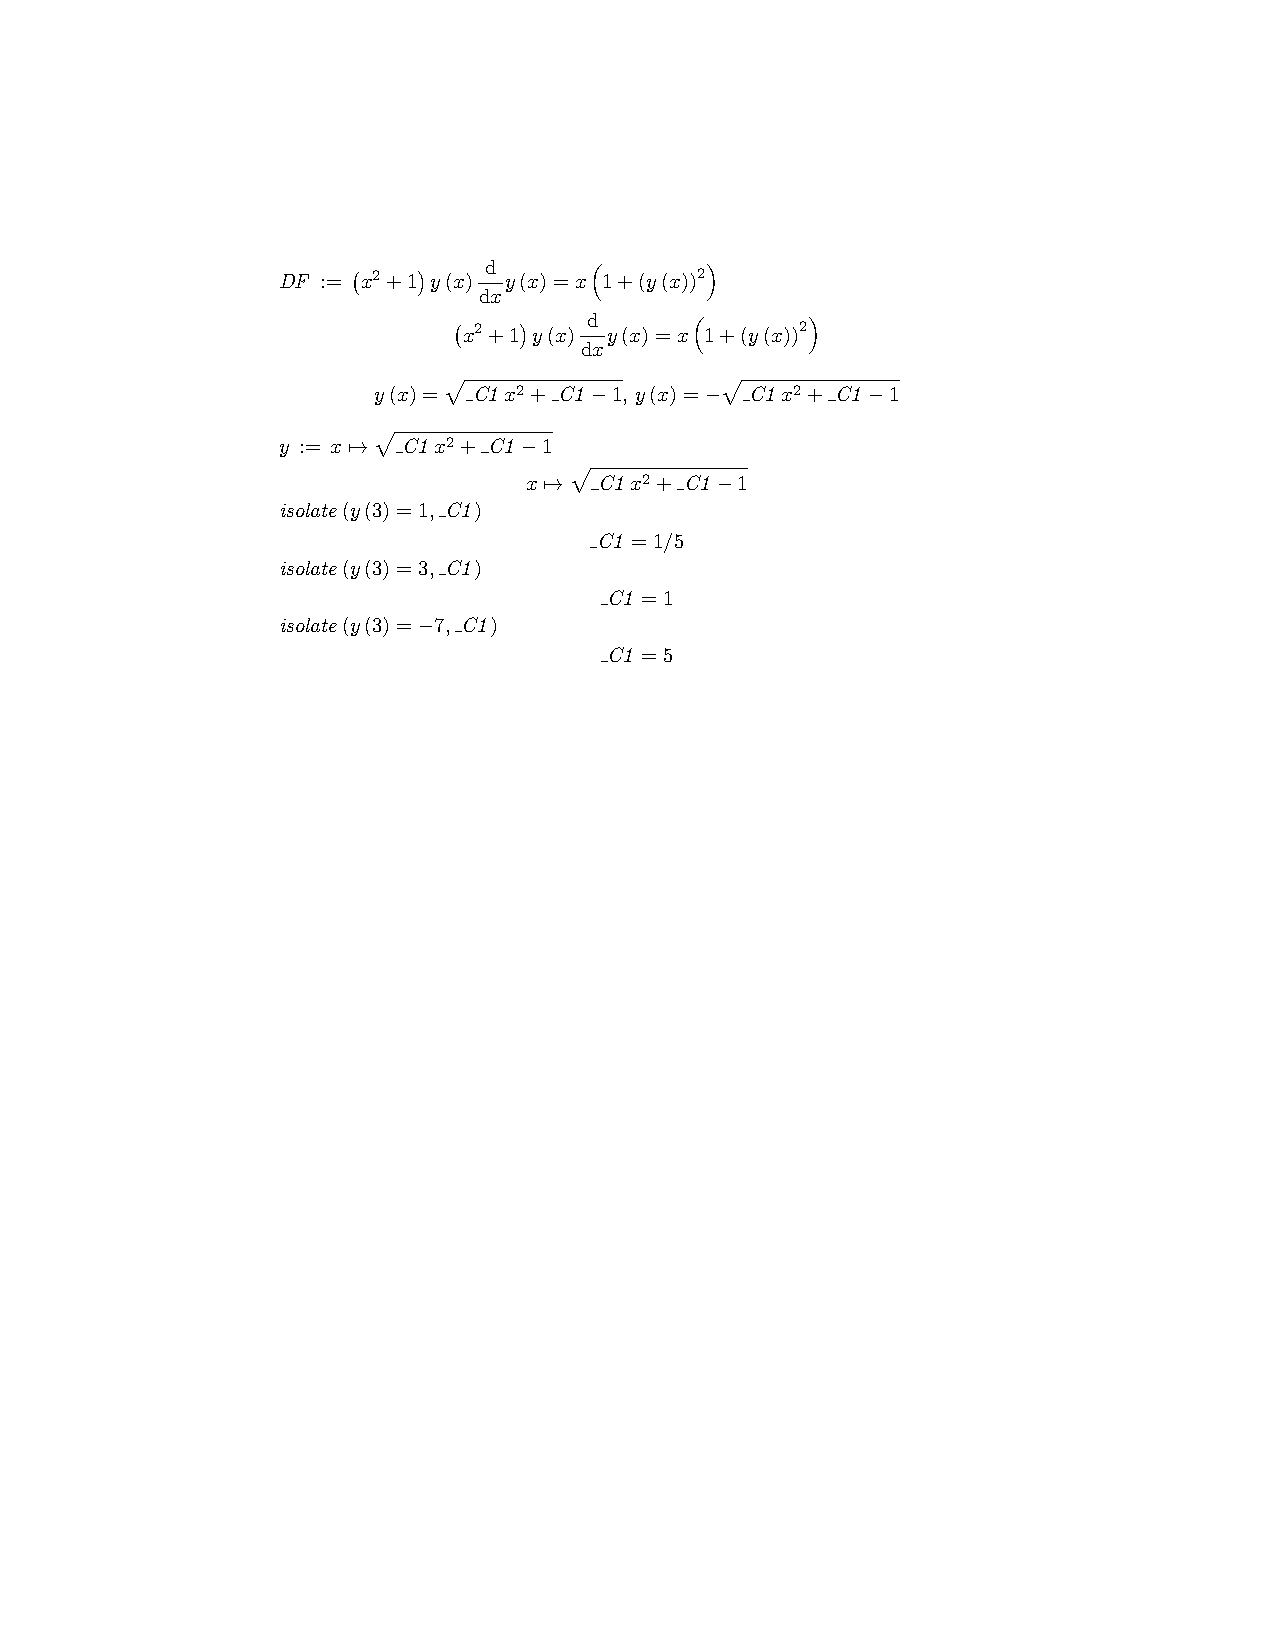
\includepdf[pages=1]{4_1_maplesolve}
\end{center}
\end{figure}
For at løse \eqref{eq:4_1} ses det at separation kan benyttes på ligninger af formen:
\begin{equation}
\label{eq:separable}
q(x)y'=p(x)
\end{equation}
At ligningen er separabel henviser til at lighedstegnet separere de to variable $x$ og $y$.
\begin{align*}
& (1+x^2)yy'=x(1+y^2) & /(1+x^2)y\\
& \Rightarrow  y'=\frac{x(1+y^2)}{y(1+x^2)} & /\frac{(1+y^2)}{y} \\
& \Rightarrow \frac{y'y}{1+y^2}=\frac{x}{1+x^2} & \text{ flyt } y' \text{ ud af brøken} \\
& \Rightarrow y'\frac{y}{1+y^2}=\frac{x}{1+x^2} & \text{ \eqref{eq:separable} er nu opfyldt} \\
& \Rightarrow \int y'\frac{y}{1+y^2} dx=\int \frac{x}{1+x^2}dx
\end{align*}
Ved dette trin kan det udnyttes at $y'=\frac{dy}{dx}$ og notationen kan misbruges til at opsætte $dy=y'dx$, dette tillader nu at udbytte ovenstående udtryk for istedet at have integralet med hensyn til $y$ således at
\[
\int\frac{y}{1+y^2}y'dx\Leftrightarrow \int \frac{y}{1+y^2} dy
\]
og det kan således indsættes således at 
\[
\int \frac{y}{1+y^2} dy = \int \frac{x}{1+x^2}dx
\]
For at løse dette kan integration ved substition benyttes. Substitution kan benyttes på integraler på formen:
\begin{equation}
\label{eq:substitution}
\int f(g(x))g'(x)dx
\end{equation}
Ved lade $u=g(x)=y^2+1$ da er $g'(x)=2y$ og det ses at ved at faktorisere brøken med $\frac{1}{2}$ og flytte udenfor integralet fås netop en funktion som opfylder \eqref{eq:substitution}, hvilket er vist i det følgende:
\begin{align*}
&\int \frac{y}{1+y^2}dy= \frac{1}{2} \int \frac{2y}{1+y^2}dy \\
& \Rightarrow \frac{1}{2} \int \frac{2y}{u}dy & \text{ Da } 2y=\frac{du}{dy} \Leftrightarrow dy=\frac{du}{2y} \\
& \Rightarrow \frac{1}{2} \int \frac{2y}{u}\cdot \frac{du}{2y}   \\ 
& \Rightarrow \frac{1}{2} \int \frac{du}{u} \\
& \Rightarrow \frac{1}{2} \int \frac{1}{u}\ du\\
& \Rightarrow \frac{1}{2}\ ln(|u|) + C & \text{ Ved at substituere } y^2+1 \text{ istedet for } u \text{ fås}\\
& \Rightarrow \frac{1}{2}\ ln(|y^2+1|) + C  & \text{ da } y^2+1 \text{ kun kan være positivt}\\
& \Rightarrow  \frac{1}{2}\ ln(y^2+1) + C
\end{align*}
Ved at have integreret den venstre side af det oprindelige udtryk og notere at venstre er identisk med højre med undtagelse af variablen kan udtrykket altså skrives som:
\[
\frac{1}{2}\ ln(y^2+1) + C_1 = \frac{1}{2}\ ln(x^2+1) + C_2
\]
$C_1 \text{ og } C_2$ er vilkårlige variable og kan samles  under en vilkårlig variabel $C_3=C_2-C_1$ på højre side.
\[
\frac{1}{2}\ ln(y^2+1) = \frac{1}{2}\ ln(x^2+1) + C_3
\]
For at isolere $y(x)$ 
\begin{align*}
&\frac{1}{2}\ ln(y^2+1) = \frac{1}{2}\ ln(x^2+1) + C_3 & \text{Gange begge sider med } 2\\
& \Rightarrow ln(y^2+1) = ln(x^2+1) + C_3 & \text{Opløft e med begge sider} \\
& \Rightarrow e^{ln(y^2+1)} = e^{ln(x^2+1)+C_3} \\
& \Rightarrow y^2+1=e^{C_3}(x^2+1)	& e^{C_3}\text{ er blot en anden vilkårlig variabel, lad } C=e^{C_3}\\
& \Rightarrow y^2+1=C(x^2+1) & \text{Træk $1$ fra begge sider} \\
& \Rightarrow y^2 = C(x^2+1)-1 & \text{Tag roden af begge sider} \\
& \Rightarrow y = \sqrt{C(x^2+1)-1}
\end{align*}
Dermed er $y(x)$ fundet til
\[
y(x) = \sqrt{C(x^2+1)-1}
\]
Da kan med udgangspunkt i hver af de givne startværdier, $c$ findes et $C$ således at $y(c)=d$ hvor $d$ er de angivne værdier stillet i opgaven. \\
For $y(3)=1$ fås:
\begin{align*}
&1=\sqrt{C(3^2+1)-1} \\
& \Rightarrow 1=\sqrt{C10-1} \\
& \Rightarrow 1 = C10-1 \\
& \Rightarrow 2 = C10 \\
& \Rightarrow C = \frac{2}{10} = \frac{1}{5}
\end{align*}
%
$y(x)=\sqrt{\frac{1}{5}(x^2+1)-1}$ \\\\
%
Ligeledes for $y(3)=3$:
\begin{align*}
&3=\sqrt{C(3^2+1)-1} \\
& \Rightarrow 3=\sqrt{C10-1} \\
& \Rightarrow 9 = C10-1 \\ 
& \Rightarrow 10 = C10 \\
& \Rightarrow C = \frac{10}{10} = 1
\end{align*}
%
$y(x)=\sqrt{(x^2+1)-1}$ \\\\
%
Og til sidst samme fremgangsmåde for $y(3)=-7$
\begin{align*}
&-7=\sqrt{C(3^2+1)-1} \\
& \Rightarrow -7=\sqrt{C10-1} \\
& \Rightarrow 49=C10-1 \\
& \Rightarrow 50 = C10 \\ 
& \Rightarrow C = \frac{50}{10} = 5
\end{align*}
%
$y(x)=\sqrt{5(x^2+1)-1}$\\\\
%
\section*{4.2 (i)}

\subsection*{b)}
%% indsæt maple her:
\begin{figure}[H]
\caption{Maple input og output }
\begin{center}
%\input{%maple fil navn} % fjern kommentering og indsæt .tex filnavn med maple tex export
\end{center}
\end{figure}



\end{document}